\documentclass[10pt,a4paper]{article}
\usepackage[T1]{fontenc}
\usepackage[scaled]{helvet}
\usepackage{cite}
\usepackage{url}
\usepackage{graphicx}
\usepackage{float}
\usepackage{amsmath}
\usepackage{amssymb}
\usepackage{fancyhdr}
\usepackage{lastpage}
\floatstyle{boxed} 
\restylefloat{figure}
\renewcommand*\familydefault{\sfdefault}
\title{Introduction to Operating Systems}
\author{David Lynch - david.lynch@raglansoftware.com }
\begin{document}
\maketitle
\begin{abstract}
In this article we step up from the physical hardware of the computer system and focus on the operating system, or where hardware meets software, meets the user. We take a look at the general structure of an operating system, some considerations when designing operating systems and define the roles and responsibilities of operating system software. There are a number of schools of thought on how operating systems should be designed and to illustrate the engineering problem, we look at a couple of approaches. 
\end{abstract}
\section{Introduction}
Formally, an operating system is a program that manages computer hardware. It provides a basis for application programs, such as word processors, by acting as an intermediary between the user and this hardware. Operating systems are found in wide ranges of computer driven devices. Each of these devices will have different important characteristics for which the operating system will be tailored. For example a main-frame controlled by OS 2200 Unisys will be engineered to cater for job execution and throughput, together with support for  multiple client users all managing the system. A personal computer system running Windows is tailored for user experience and responsiveness. An embedded real-time operating system such as LinuxOS RTOS is engineered to provide guarantees around how long computations will take. Lastly, a mobile operating system such as iOS6 will be optimized for user experience, power consumption and cater for various modes of interaction typically not supported by a personal computer.
\subsection{Perspectives}
Each of the above examples can be examined in terms of the user or the system perspective. A microcomputer is designed for ease of use and responsiveness with little attention given to resource utilization. 


\begin{figure}
\caption{Abstract view of an operating system. \cite{OSCONCEPTS}}
\begin{center}
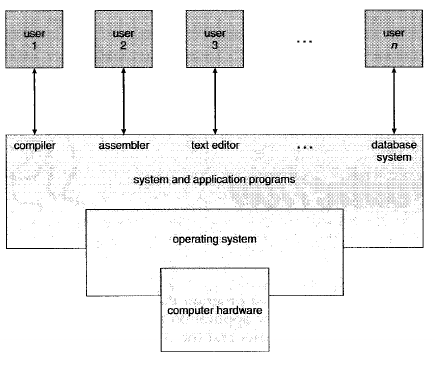
\includegraphics[scale=0.45]{../images/operating-system.png}
\label{memory-h}
\end{center}
\end{figure}

\bibliography{../biblio/techfundamentals.bib}{}
\bibliographystyle{plain}
\begin{center}
{\small \copyright  David Lynch 2012. Do not reproduce with written permission.}
\end{center}
\end{document}